%!TEX root = ../main.tex

\section{Attacks on bitcoin mining}
In Section~\ref{sec:fork} we have shown that continued forks are
extremely unlikely, if nodes stick to the longest chain rule and
do not disturb the network latency.

In the following we first look at two ways to deviate from the 
longest chain rule, stubborn mining and selfish (hidden) mining.
And we look at network attacks that might be performed.

We first look at those attacks from the perspective of fair mining.
Then we look at them from the perspective of a double spend.

\begin{definition}
Mining, or block creation is \emph{fair} if a node that possesses $\alpha$ 
percent of the hashing power in the network ends up publishing $\alpha$
blocks in the longest chain.
\end{definition}


\subsection{Stubborn mining}
A node does perform stubborn mining, if it does not abandon the 
current chain for the longest chain. Thus it does not follow the longest chain rule.

More precisely, if there exist two blockchains $c_1$ and $c_2$ 
and $c_2$ contains one more block than $c_1$. Thus the initial state is as shown in Figure~\ref{fig:fork}.
A stubborn node that has published a block in $c_1$ that is not
part of $c_2$ will continue to try and extend $c_1$ until either
$c_1$ becomes the longest. We assume that if the difference between
$c_1$ and $c_2$ increases, the stubborn node will abandon $c_1$.

\begin{theorem}
	
	Stubborn mining does not increases the expected outcome of a node, if
	the node controls less than $\alpha=0.42$ of the hashing power in the network.
	
\end{theorem}
\begin{proof}
	We model this system as a markov chain with 4 states.
	\begin{itemize}
		\item[Loose] where chain $c_1$ was extended faster than $c_2$.
		\item[$-1$] where chain $c_1$ is one block longer than chain $c_2$.
		\item[$0$] where $c_1$ and $c_2$ are equally long.
		\item[Win] where chain $c_2$ became the longest chain.
	\end{itemize}
	
	We ignore the probability that additional forks occur on $c_2$ but 
	note that they would increase the profitability of stubborn mining.
	Assume the probability that the attacker finds a block is $\alpha$,
	while $\beta=1-\alpha$ is the probability that the remaining miners find a block. The states and the transition probabilities are shown in Figure~\ref{fig:stubborn}.
	\begin{figure}
	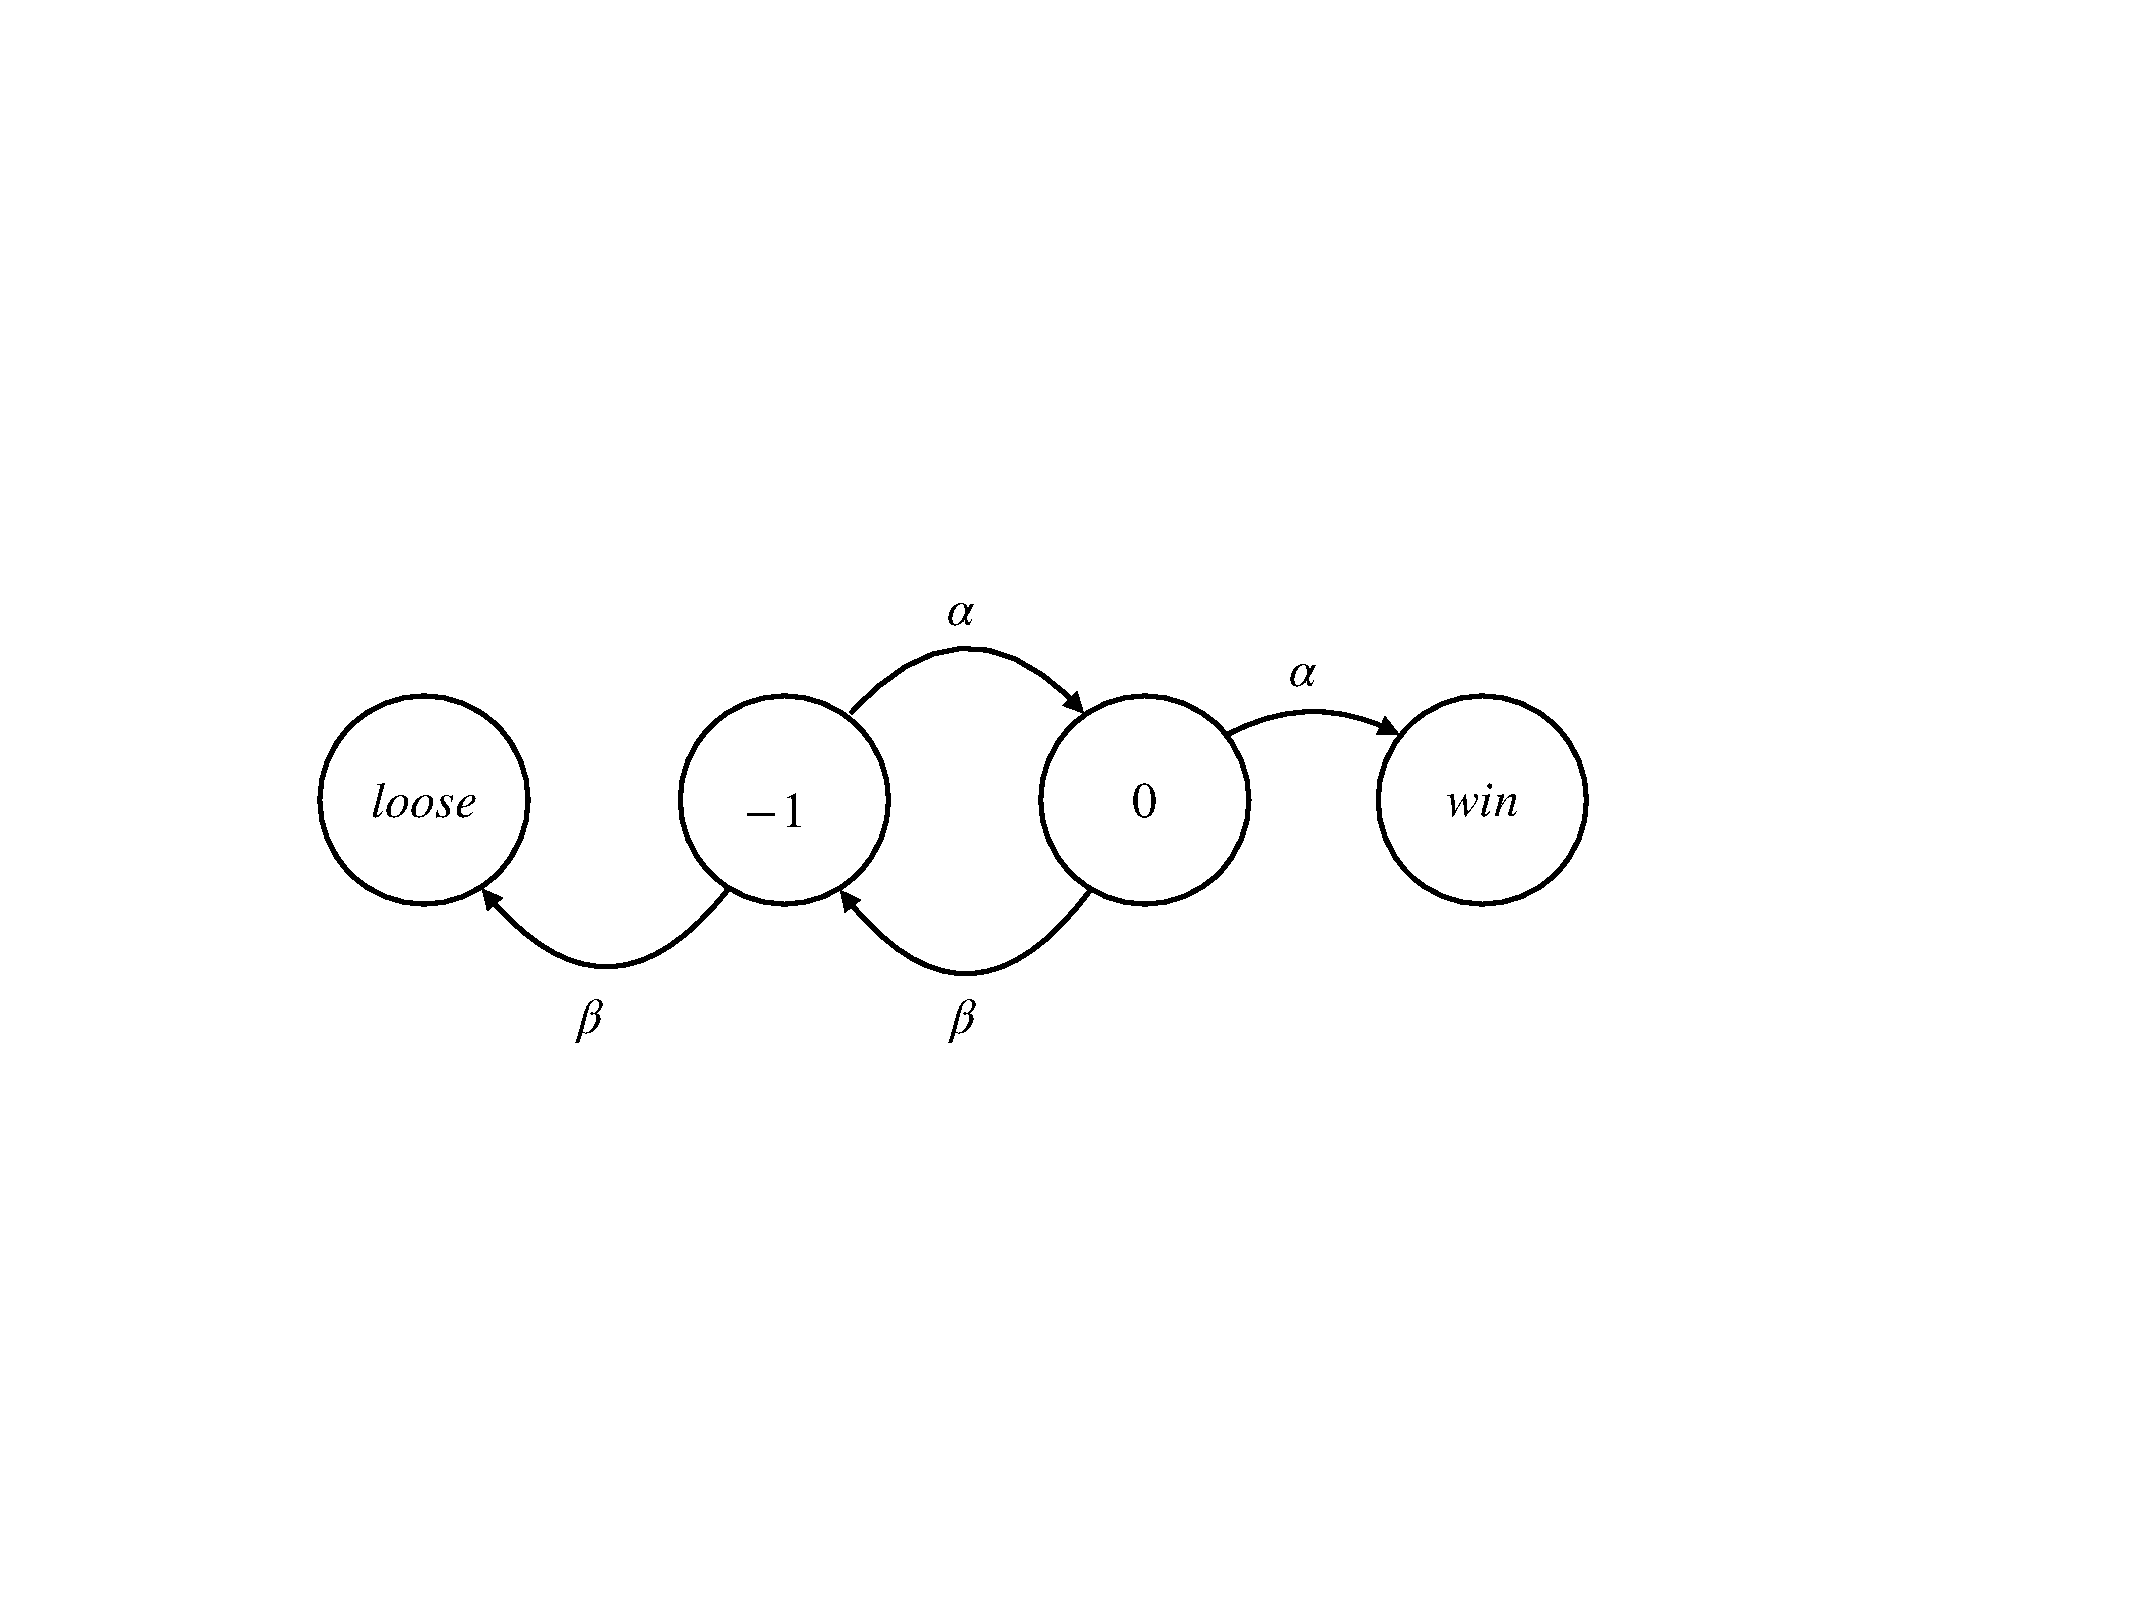
\includegraphics[width=\textwidth]{fig/StubbornMining}
	\caption{Stubborn mining states and transitions.}
	\label{fig:stubborn}
	\end{figure}
	
	We now calculate the expected number of blocks the Attacker receives with and without doing the attack. 
	For the attack we consider the following cases:
	\begin{itemize}
		\item With probability $\beta$ the attacker loses in the first step and receives no blocks.
		\item With probability $\alpha\cdot \alpha$ the attacker mines two blocks. He receive 3 blocks in total.
		\item With probability $\alpha\cdot\beta\cdot \alpha\cdot \alpha$ the process goes through states $-1\mapsto 0 \mapsto -1 \mapsto 0 \mapsto win$.
		In this case the attacker gets 4 blocks.
	\end{itemize}
	Extending the above cases, and omitting those that give 0 blocks,
	$E_{Attack}$ the expected number of blocks is:
	\begin{align}
		E_{Attack}&=\sum_{i=0}(i+3)\alpha^{i+2}\beta^{i}\\
				  &=3\alpha^2+\alpha\beta\left(\sum_i=0(i+3)\alpha^{i+2}\beta^i +\sum_{i=0}\alpha^{i+2}\beta^i\right)\\
				  &=3\alpha^2+\alpha\beta\left(E_{Attack} +\frac{\alpha^2}{1-\alpha\beta}\right)
	\end{align}
	In step (3.2) we used the formula for a geometric sum.
	Solving the above for $E_{Attack}$ gives
	\[
		E_{Attack}=(3+\alpha\beta)\frac{\alpha^2}{1-\alpha\beta}
	\]
	
	To compute the average number of blocks, the attacker would receive if it did not follow the attack, we note that the he gets one block every time an edge with probability $\alpha$ is traversed. We get the following cases.
	\begin{itemize}
		\item With probability $\alpha\cdot \alpha$ the node mines two blocks.
		\item With probability $\alpha\cdot\beta\cdot \beta$ the process goes through states $-1\mapsto 0 \mapsto -1 \mapsto loose$. The node mines 1 block.
		\item With probability $\alpha\cdot\beta\cdot \alpha\cdot \alpha$ the process goes through states $-1\mapsto 0 \mapsto -1 \mapsto 0 \mapsto win$.
		In this case the node gets 3 blocks.
	\end{itemize}
	Continuing the above analysis, we see that the average number of blocks received when not following the above state machine, but not following the attack, is:
	\[
	E_{NoAttack}=\sum_{i=0}(i+2)\alpha^{i+2}\beta^i + \sum_{i+0}i\beta^{i+1}\alpha^i
	\]
	Using the same techniques as for $E_{Attack}$, we get:
	\[
	E_{NoAttack}=(2+\alpha\beta)\frac{\alpha^2}{1-\alpha\beta}+(1+\alpha\beta)
	\]
	
	Plotting both graphs we see that $E_{Attack}<E_{NoAttack}$ holds approximately for $\alpha<0.42$.
\end{proof}

\subsection{51\% attack}
If a miner owns $\alpha=51\%$ of the hashing power in the network, he can attack the network by creating and growing his private chain.
Key to this attack is that the attacker will be able to grow his private chain faster than the remaining network can grow the public chain.

\begin{example}
This example is shown in Figure~\ref{fig:51}. 
Assume at the begin of the attack the longest chain contains blocks $b_1$, $b_2$, and $b_3$. The attacker picks a recent block, e.g. $b_2$ and starts secretly extending $b_2$. Once the attacker has extended his chain longer than the public chain he can publish it and all blocks in the public chain will be discarded.
\end{example}

\begin{figure}
	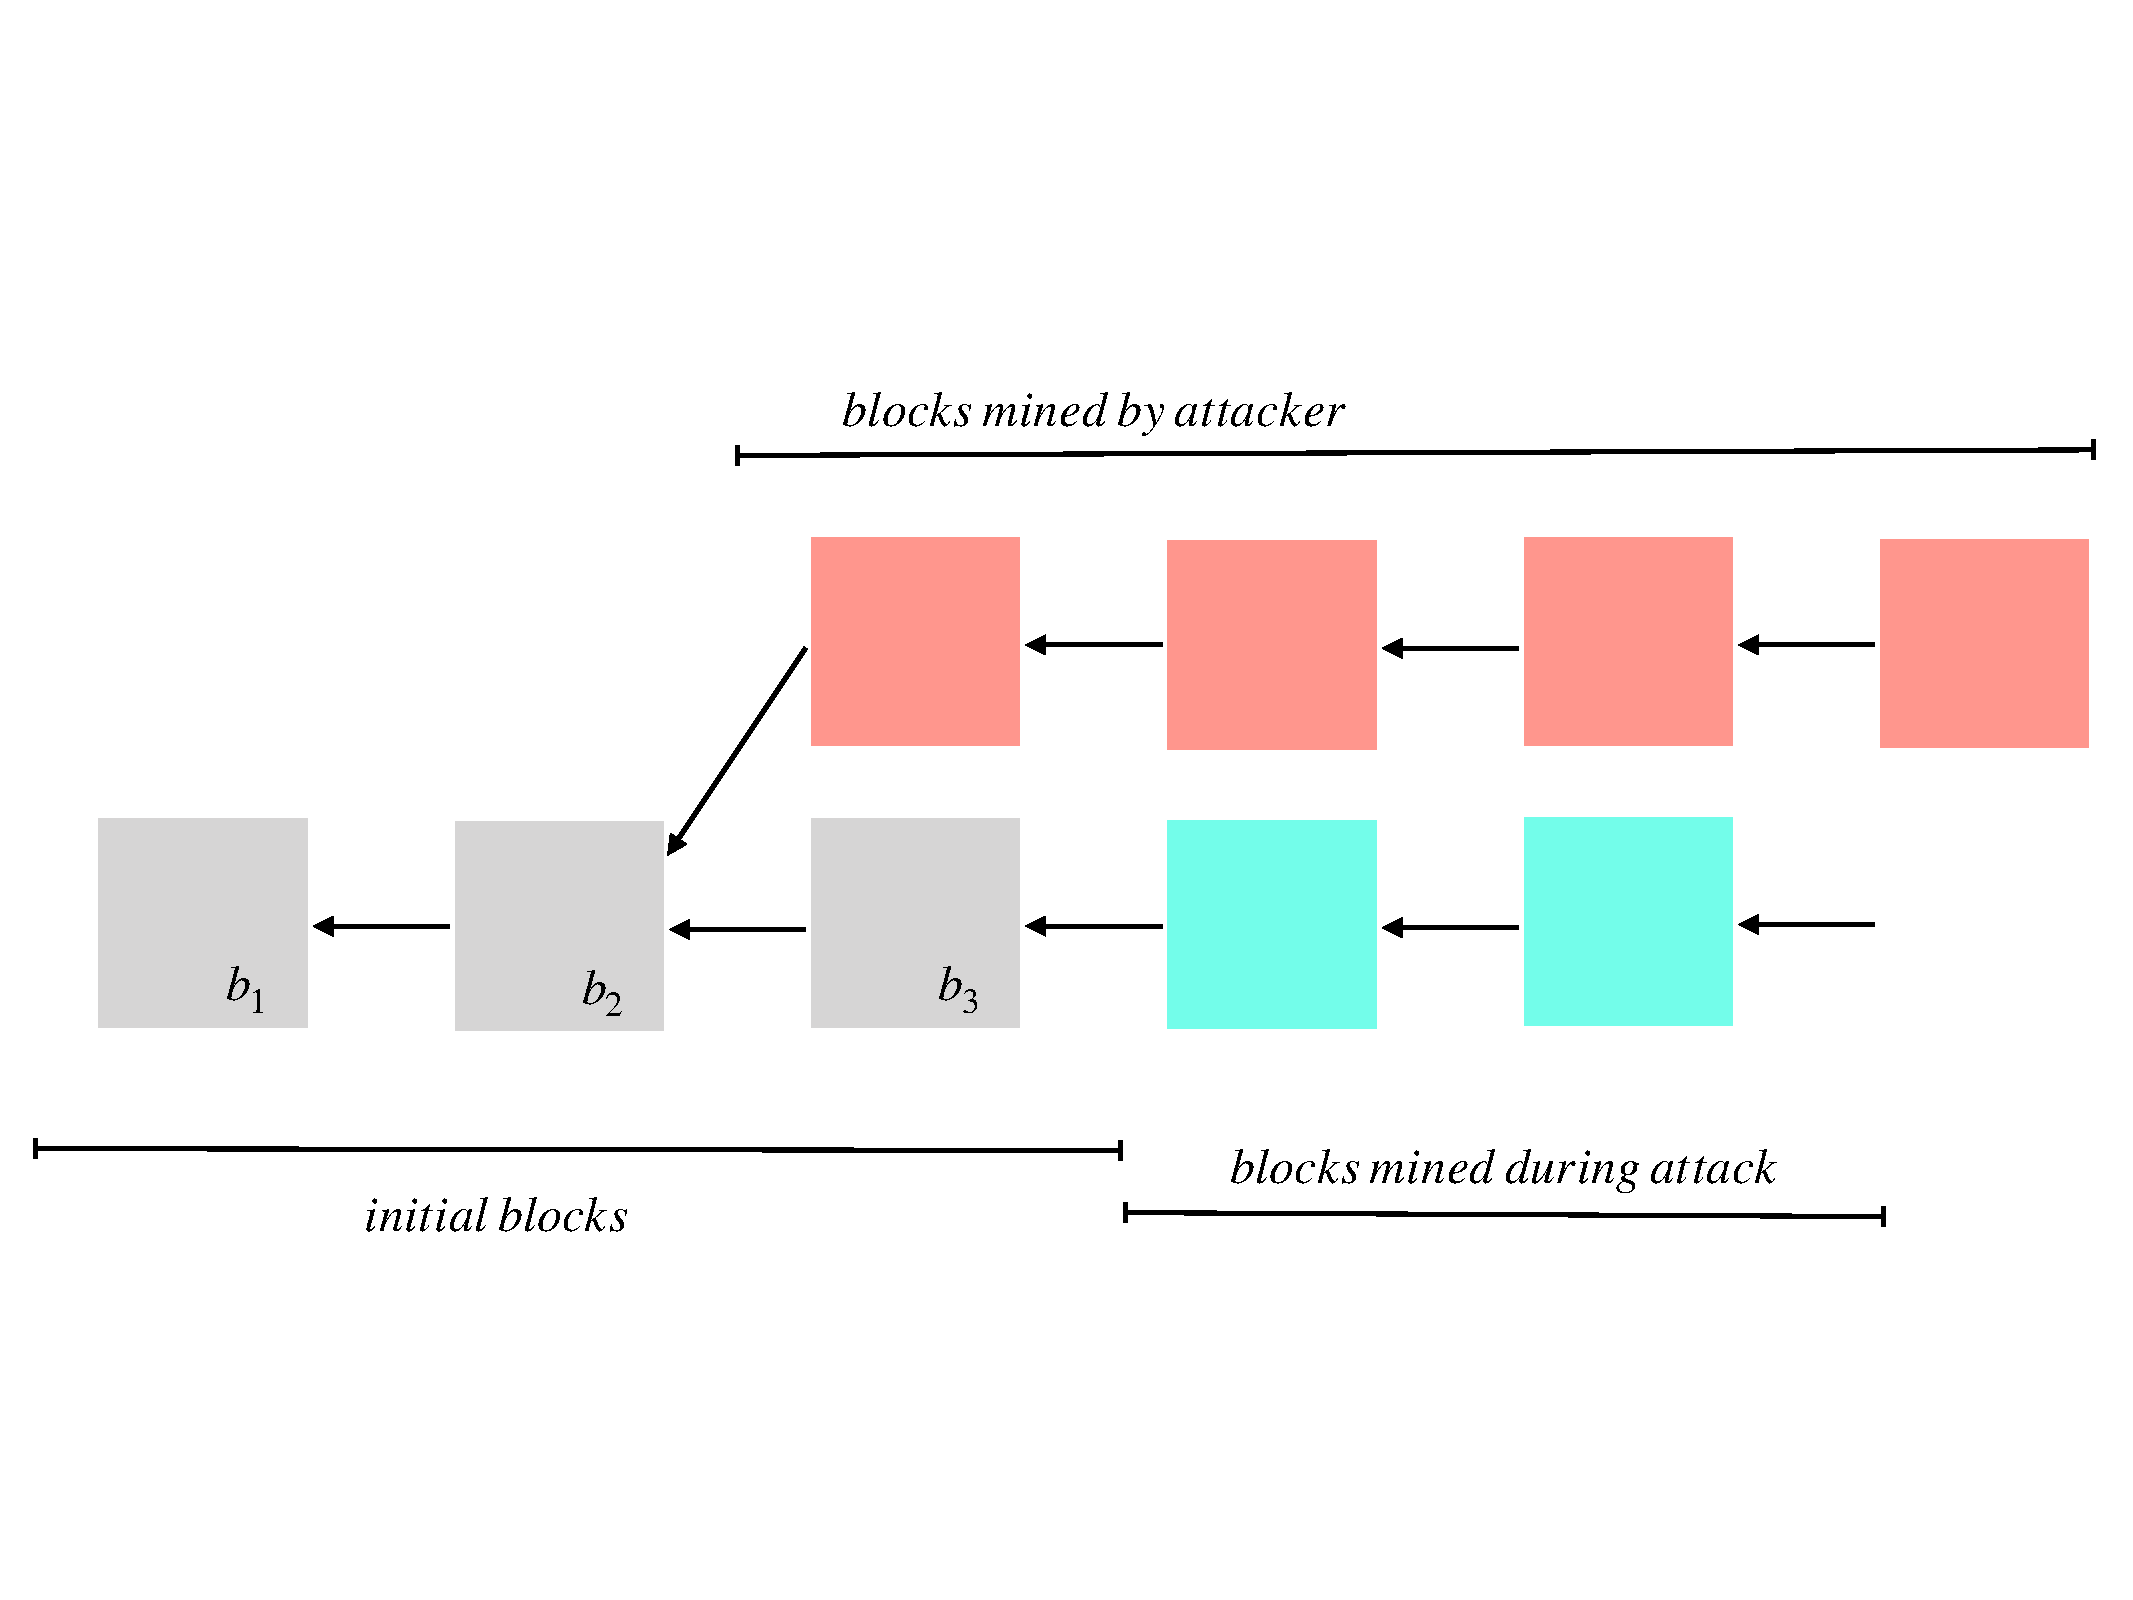
\includegraphics[width=\textwidth]{fig/51attack}
	\caption{A 51\% attack.}
	\label{fig:51}
\end{figure}

\subsection{Selfish mining}
In a selfish mining attack, the attacker does not violate the longest chain rule. Instead he violates the following mandate:
\begin{description}
	\item[Publication mandate] When a node finds a block, it should immediately announce this to the other processes. 
\end{description}
The idea behind not publishing the newest block is that it denies the other nodes to try and extend the longest chain. Thus, other nodes waist resources, trying to extend a chain, that is not the longest chain.

For a detailed description and analysis of selfish mining see 
 \href{https://disco.ethz.ch/courses/distsys/lnotes/chapter26.pdf}{Chapter 26.1} of these Lecture notes form ETH Zurich.
 
\begin{note}
Results above show, that, if the attacker has more than $1/3$ of the hashing power, he can increase the ratio of blocks he creates in the blockchain by selfish mining.

\begin{itemize}
	\item If the attacker has more than $\alpha=1/3$ of the hashing power, he can increase the ratio of blocks he creates in the blockchain by selfish mining.
	\item If the attacker has more than $\alpha=1/4$ of the hashing power, and can reach $\gamma=0.5$ half of the nodes before another miner can reach them, he can benefit from selfish mining.
\end{itemize}
\end{note}

\section{P2P networking and network layer attacks}
A node in bitcoin does not maintain connections to all 10.000 bitcoin nodes.
Instead every node maintains a membership list, with addresses of other nodes. He maintains connections only to a few nodes selected at random from the list. 
We say that these connections form an overlay network.

In Bitcoin, nodes per default start by establishing 8 connections and extend this to up to 125 connections.

When a block is broadcast, every peer receiving the block first validates it and then forwards it to its neighbors. 

\subsection{Inventory messages and delivery denial attack}
The forwarding of a block consumes significant bandwidth. 
Bitcoin therefore uses \textsc{Inventory} messages to announce the a block to neighbors. Receiving an \textsc{Inventory} message a node would request to receive the actual message from only one of its neighbors. 

Nodes set a timeout when requesting a block. If they do not receive the block within the timeout, it is requested from a different source.

\begin{itemize}
	\item In bitcoin version 0.10, the timeout for receiving a block is set to 20 minutes.
\end{itemize}

\begin{definition}
In a \emph{delivery denial attack} a node does send \textsc{Inventory} messages, but when a block is requested, does not forward the block.	
\end{definition}

For extended details on this attack, see \href{https://scalingbitcoin.org/zh_HANS/papers/bitcoin-block-transaction-delivery.pdf}{[Gervais et. al. in CSS'15]}.
\question{What is the effect of this attack?}

\begin{note}
	Due to the static timeout, a delivery denial attack can significantly slow down block propagation.
	
	\begin{itemize}
		\item Slowing delivery of blocks increases the probability of a fork, as can be seen from Theorem~\ref{thm:fork}. This also increases the probability that a fork extends for several blocks.
		\item Slowing delivery of competing blocks may increase parameter $\gamma$ in the selfish mining scheme and thus make selfish mining more appealing and profitable even when $\alpha<1/4$.
	\end{itemize}
	
\end{note}

\subsection{Eclipse attack}




\section{Updating a blockchain}

\section{Pow as voting}